% !TEX root = ../../report.tex

\begin{comment}
Students should list the materials and instruments used in the experiment, as well as provide a
description of the overall experimental setup. It is recommended that you include a simple schematic
drawing of the setup (no photos of the setup).
\end{comment}
In this section a brief illustration of the experimental setup is provided.
Before, a list of the materials used follows:
\begin{enumerate}[label=\alph*)]
\item \label{item:breadboard} aluminum optical breadboards;
\item posts, mounts and supports for the optical elements;
\item \label{item:half_wave} mounts for wave plates and 4 $\lambda
  /2$ wave plates, with
  indication of the angles;
\item \label{item:pbs} 2 polarizing beam splitters (PBS);
\item \label{item:laser} 2 \SI{635}{\nano \meter} laser diodes;
\item electronics to control the lasers;
\item \label{item:detectors} 4 laser pulse detectors and respective electronics;
\item screwdivers and instruments to assemble the setup;
\item \label{item:card} aligner card, sensitive to laser light;
\item \label{item:attenuators} laser curtains and beam stoppers.
\end{enumerate}

Before starting with the discussion, let's state clearly that all the
operations necessary
to align the elements, like
lasers and beam splitters, are performed live during the construction
of the setup. These actions are
always carried out with the help of rulers, to check for the height of the
different entities, and with the cardboard piece
\cref{item:card} to align the
laser beam without having to
rely only on geometrics considerations.
Another important disclaimer regards the fact that during the whole
experience all the laser paths were terminated either by a detector
\cref{item:detectors}
or by a beam stopper \cref{item:attenuators}, to avoid uncontrolled
free beams inside the room.
Those two operation will be assumed done at all times, and so they
will not be cited consistently during the following discussion.

The first operation involved the understanding of the laser's emitted
radiation polarization with respect
to the laboratory's frame of reference.
To do that, the laser \cref{item:laser} and its post were assembled
and fixed to the
optical table. A polarizing beam splitter \cref{item:pbs} was then
put in front of it to
intercept the light.
As said previously, before turning on the laser, stopper are placed
to limit light propagation. Then the laser was turned on and a mobile
ruler was used to control the propagation direction with respect to
the optical table plane. The setup was then fixed with the laser beam
parallel to that plane.

The physical situation obtained is depicted schematically in
\cref{fig:qkd_beam_real}.
At this point, the polarization of the light is not known to the
experimenters. The only clear information is that the laser
effectivly emit a linearly polarized light.
To fix the polarization, the laser was rotated around
its longitudinal symmetry axis.

\begin{figure}
\centering
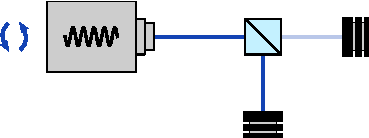
\includegraphics[height=2cm]{./qkd/bb84/images/laser_polarization_calibration_real.pdf}
\caption{Example of a starting position for laser calibration.}
\label{fig:qkd_beam_real}
\end{figure}

\begin{figure}[h]
\centering
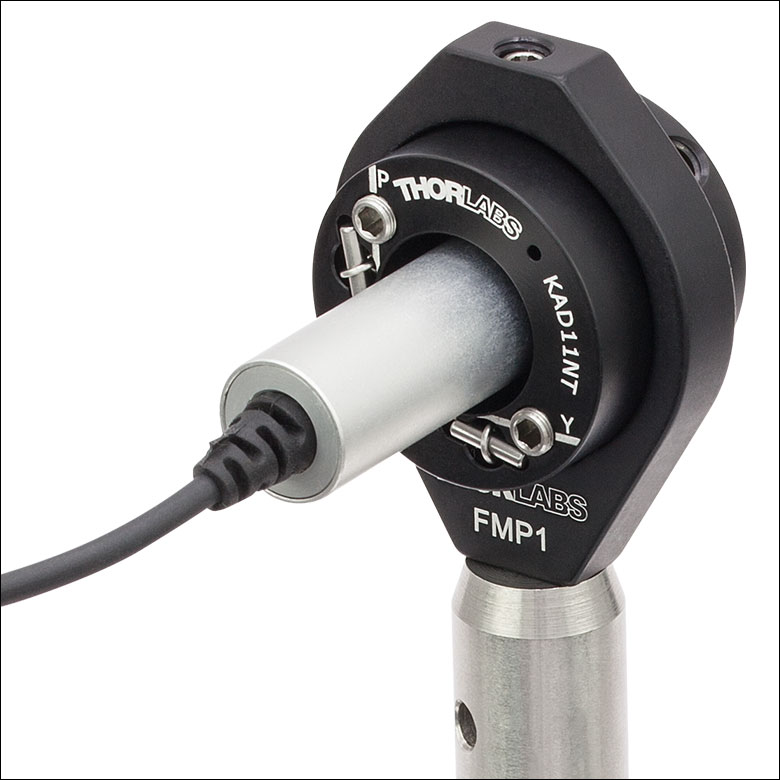
\includegraphics[height=4cm]{../bb84/images/laser_in_post.png}
\caption{An example of the laser and the post on which it was fixed on.
Image taken from \href{https://www.thorlabs.com}{Thorlabs}.}
\label{fig:laser_post}
\end{figure}
An example of the laser and its post is shown in \cref{fig:laser_post}.

Since the beam splitter is a polarizing one, it separates the
incoming light depending on its polarization.
In particular, as seen in \cref{fig:PBS}, the splitter used let through
light with horizontal polarization, while reflecting the vertically
polarized one. The directions are meant with respect to the optical
breadboards \cref{item:breadboard}
placed parallel to the floor.

\begin{figure}[h]
\centering
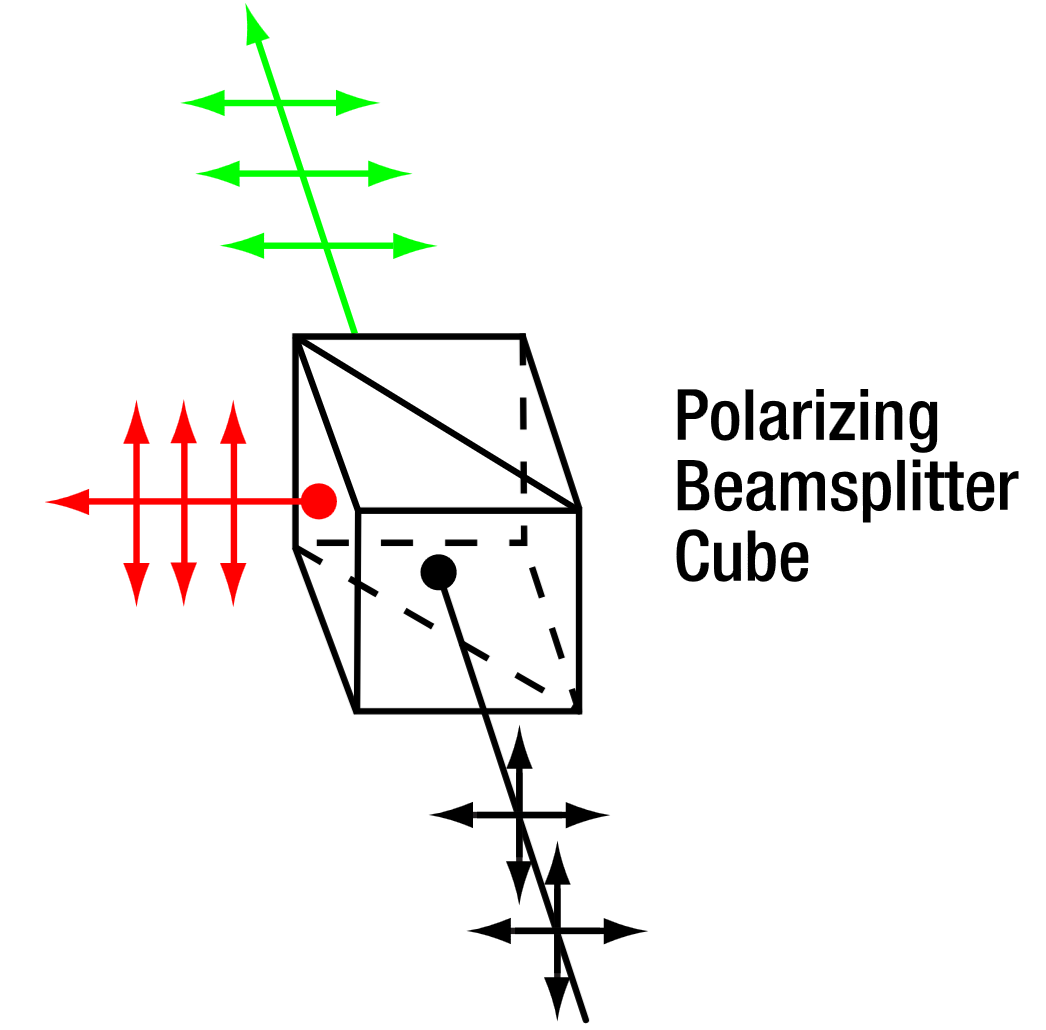
\includegraphics[height=4cm]{./qkd/bb84/images/pbs.png}
\caption{Schematic view of polarization discrimination by a
  polarizing beam splitter.
Image taken from \href{https://www.thorlabs.com}{Thorlabs}.}
\label{fig:PBS}
\end{figure}

Since the starting beam was choosen to be a vertically polarized one,
the laser underwent a rotation until all the light went through the
reflected arm, like in \cref{fig:qkd_beam_perfect}.

\begin{figure}
\centering
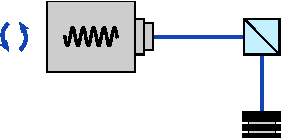
\includegraphics[height=2cm]{./qkd/bb84/images/laser_polarization_calibration_ideal.pdf}
\caption{Target setup scheme for laser calibration.}
\label{fig:qkd_beam_perfect}
\end{figure}

Notice that, during this procedure, since the human eye can
discriminate better differencies in low light intensity
\cite{goldstein2014sensation}, the
transmitted beam's intensity was monitored and minimized visually.
In the end, after removing the beam splitter the light can be
confidently assumed to be vertically polarized with respect to the
optical table's plane; that means that the plane where the
electromagnetic field oscillates is the one perpendicular to the
optical table's plane.
Notice that the word confidently was used: that is referred to the
fact that the carried minimization didn't allow to completely dim the
transmitted beam, indicating possible defects either in the PBS light
splitting or a big uncertainty in the laser's claimed linear polarization.

After this procedure the real experiment could begin.
The demonstration is divided in two main parts: a general
illustration of the protocol without any external attackers, and a
depiction of the simple "intercept and resend" threat.

\subsubsection{2-parties experiment}
Let's define, as usually done in literature, the two parties as Alice
and Bob, where Alice is sending the bits and Bob is receiving them.
Before diving into the setup details a theoretical discussion is
needed to clarify the protocol.
The protocol follows the original BB84 \cite{Bennett_2014} idea,
assuming the presence of a
public unprotected and unidirectional quantum channel and a
public bidirectional authenticated classical channel:
\begin{itemize}
\item Alice and Bob agree on the use of a particular two
  dimensional quantum system, that is the smallest system able to
  express quantum behaviour, a qubit;
\item Alice and Bob agree on two orthonormal basis of this system.
  They choose them in a way to maximize the disturbance made by an
  eventual attacker \cite{goldstein2014sensation}; practically in
  this case they are
  chosen in such a way to introduce an angle of \SI{45}{\degree}
  between the correspondent basis vector like in \cref{fig:basis}.
  Alice and Bob associate a classical bit (e.g. 0 or 1) to each one
  of the two basis vector, as shown again in \cref{tab:bitsassociation};

  \begin{figure}[h]
    \centering
    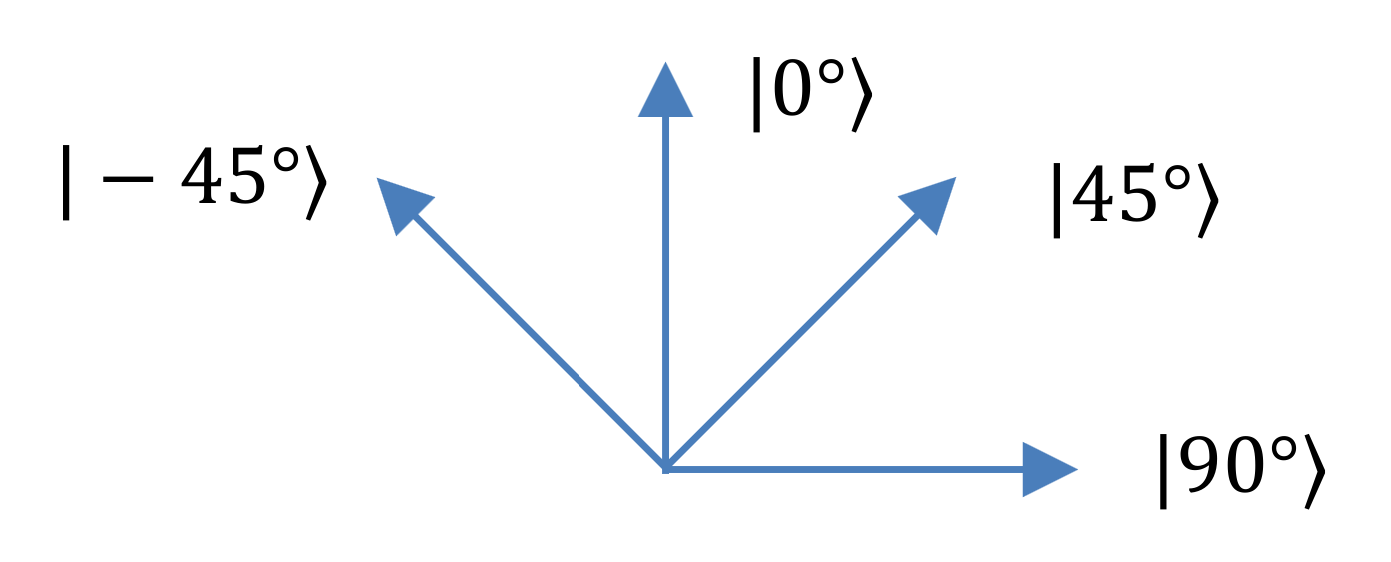
\includegraphics[height=2cm]{./qkd/bb84/images/basis.png}
    \caption{Basis choice. \textit{B1} is the one composed by the polarization
      $\ket{0°}, \ket{90°}$ and \textit{B2} by $\ket{-45°}, \ket{45°}$.
    Image taken from \href{https://www.thorlabs.com}{Thorlabs}.}
    \label{fig:basis}
  \end{figure}

  \begin{table}[h]
    \centering
    \begin{tabular}{ccc}
      \toprule
      Polarization State & Bit & Basis \\
      \midrule
      Horizontal ($\ket{90°}$)            & 0 & Rectilinear ($+$) \\
      Vertical ($\ket{0°}$)             & 1 & Rectilinear ($+$) \\
      $\ket{45°}$ (diagonal)            & 0 & Diagonal ($\times$) \\
      $\ket{-45°}$ (anti‑diagonal)       & 1 & Diagonal ($\times$) \\
      \bottomrule
    \end{tabular}
    \caption{Correspondance table between the quantum states and the
    classical bits.}
    \label{tab:bitsassociation}

  \end{table}
\item For each bit that Alice wants to send:
  \begin{itemize}
    \item Alice chooses randomly one between the two basis, for
      example using a random number generator (better if quantum);
    \item Alice generates another random bit and send the
      corresponding quantum basis state to Bob;
    \item Bob receives the quantum state, chooses a random basis
      between the two and applies a projective measurement
      according to that basis. Then he record the couple (basis, result);
  \end{itemize}
\item After receiving all the bits, Alice streams to the public
  channel the used basis, per each sent bit;
\item Bob tells back on the public channel which bits he measured
  using the same basis as Alice;
\item Both keep only the bits tagged by Bob for the key sythesis.
  This step is usually referred to as the "sifting" step.
\item The final steps will be introduced in the paragraph related
  to the eavesdropper.
\end{itemize}

Speaking about practical implementation, the two level quantum system
used here is the Hilbert space of the possible polarization of a
photon (or in this case the bunch of photons constituting the actual light).

Here other objects needs to be used to practically manipulate the
polarization, in
particular two half-wave plates \cref{item:half_wave}, its posts and supports.
The half-wave plate is an optical lens that has the ability to rotate
linar polarizations by an angle determined by the orientation of the
lens itself. A schematic is presented in \cref{fig:half_wave}.

\begin{figure}[h]
\centering
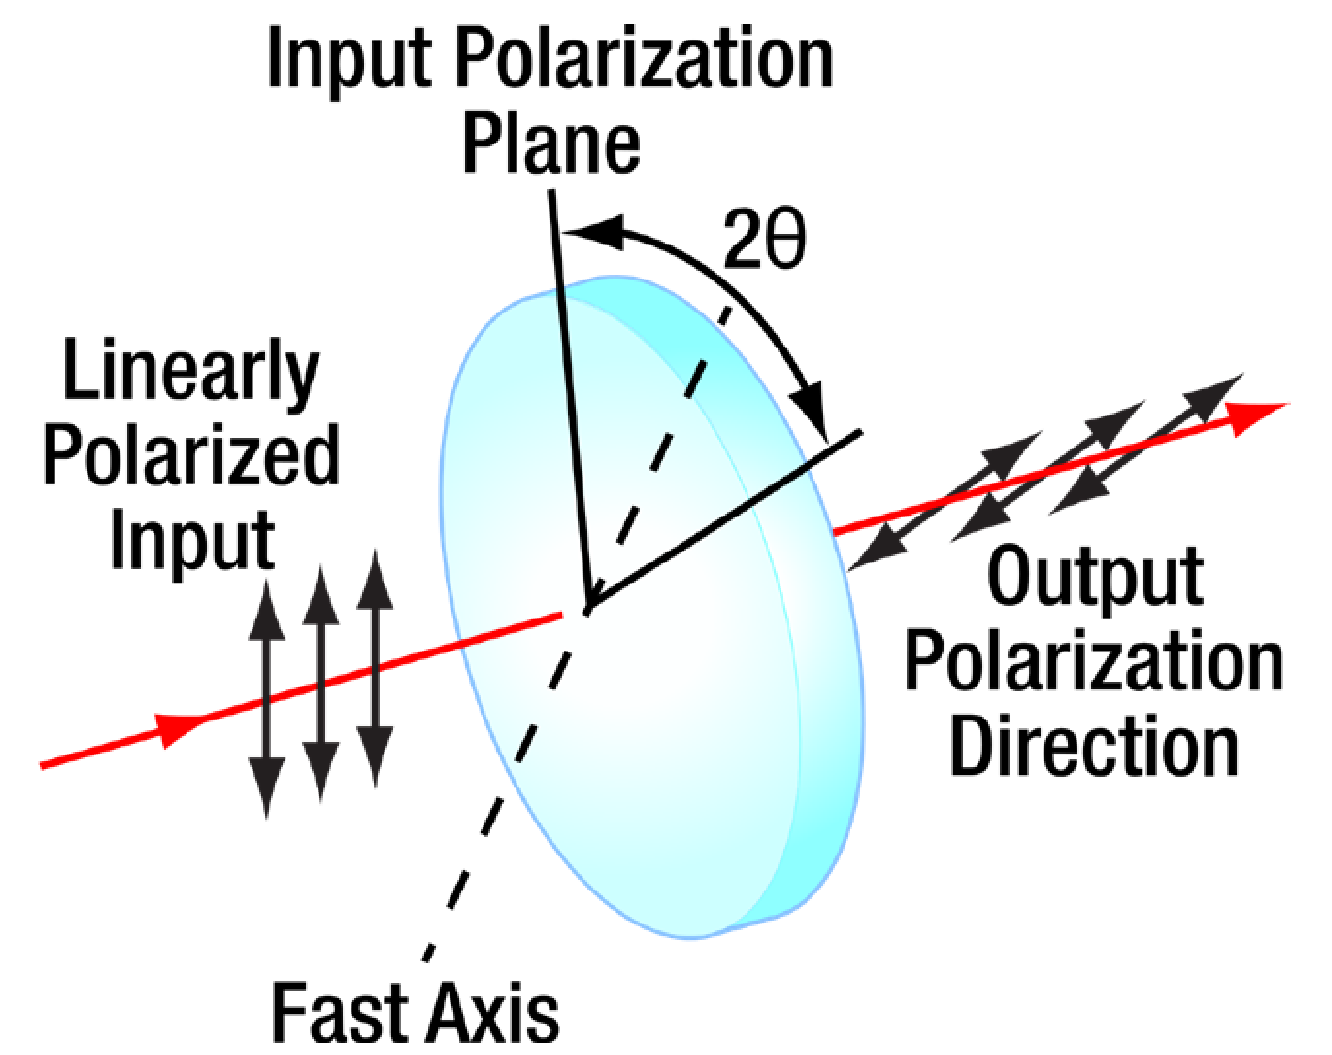
\includegraphics[height=3cm]{./qkd/bb84/images/half_wave.png}
\caption{An example of the effect of a $\lambda /2$ wave plate. Image
taken from \href{https://www.thorlabs.com}{Thorlabs}.}
\label{fig:half_wave}
\end{figure}
As can be seen, given the angle formed between the linear
polarization plane and the optical axis of the lens as $\theta$, the
output radiation's polarization is rotated by an angle $2 \theta$.

Before starting to rotate polarizations, the waveplate, shown in fig
TODO, needs to be calibrated, meaning that the optical axis needs to
be determined. Since the sent ray has an (approximately) vertical
polarization w.r.t. the optical table's plane, a polarizing beam
splitter is put after the half-wave plate and a procedure similar to
the one indicated before (TODO put a sort of scheme indicating this
repeating procedure and refer to it here) is carried out. Also in
this case the minimized ray was the transmitted one, since the
optical axis needed to be aligned to the incoming polarization, and
the origin of the angle fixed on the lens rotation mount (as shown in
TODO figure ...).

Another half-wave plate is then put spatially after the first and the
same procedure is repeated TODO(REF).

These two lenses allow respectively Alice and Bob's basis choices.

\subsubsection{Intercept and resend attack}

In this part of the experiment, a specific example of attack is
carried out supposing
that there is a third party, called Eve (for eavesdropper), trying to
gain information
on the information sent from Alice to Bob.
After choosing randomly a
basis \textit{B} between the two public ones Alice and Bob agreed on,
Eve phisically
interrupts their link (in this case a free space link, because photons
are not sent inside
the fiber) and measures
incoming light quanta performing a projective measurement on the
basis \textit{B}.
Immediately after Eve generate a state identical with respect to the
one measured and
sends it to Bob.

Notice that thanks to the no-cloning theorem [TODO:ref] Eve introduces
some disturbances to the state sent by Alice. This happens since Eve
tries to measures
a equi-weighted statistical mixture of 4 quantum states, represented
by this density matrix:
TODO:dmatrix.
that contains non orthogonal quantum states. Eve so cannot
discriminate reliably between all of them [TODO:ref].

The disturbances introduced by Eve can be detected by Alice and Bob in the
"parameter estimation" step of the protocol, where, after sifting,
they share a part of the secret bits
to check for errors, caused by noise in the instruments used,
environment or attacker side eavesdropping.
Without noise the situation is clear: no eavesdropping corresponds to
0 \% of error,
since the kept bits are the ones where Alice and Bob respectively produced and
measured states in the same basis. An eavesdropping attempt where Eve
tries to apply the
prepare and measure strategy on all the quantum states instead produces a
error rate of $25 \%$ of the sifted bits. So, taking an appropriate
sample of the sifted bits
the communicating parties can infer reasonably the presence of an attacker.
They will then abort the protocol, deeming the quantum channel unsafe
to be used.

Notice that this is only one of the various strategy that can be
employed to attack the
communication channel. Moreover, a formal security proof needs to be
carried out for more general attacker
interactions. [TODO found in ramona book].

Practically the states used here are still the polarization states
used in section
[TODO put reference of the previous section]. Eve to measure the
states uses a duplicate of the
receiver apparatus of Bob and a duplicate of the sending apparatus of Alice.
